% Figs. 5 and 6 belong to Sections III-D and IV-A; model.tex inputs this file at the
% end of III-B, so the two figures pair at the top of the next page
\begin{figure}[t]
\centering
% the ordinary policy over three kinds of step; steps from models.v lemmas
% immediate_states_no_dI / _with_dI
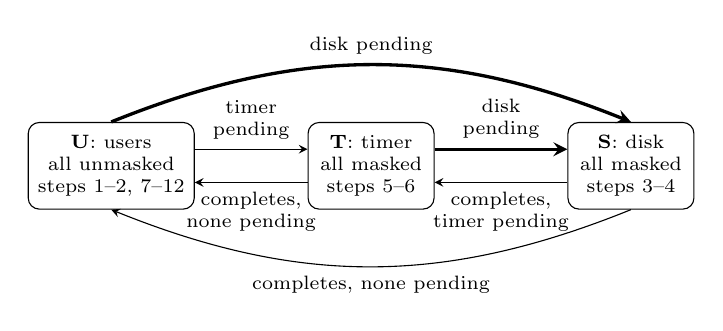
\begin{tikzpicture}[font=\scriptsize, >=stealth,
  ph/.style={draw, rounded corners, align=center, minimum width=1.6cm,
    minimum height=1.1cm, inner sep=3.5pt},
  note/.style={align=center, font=\scriptsize},
  secret/.style={->, line width=1.2pt}]
\node[ph] (u) at (0,0)   {\textbf{U}: users\\all unmasked\\steps 1--2, 7--12};
\node[ph] (t) at (3.3,0) {\textbf{T}: timer\\all masked\\steps 5--6};
\node[ph] (s) at (6.6,0) {\textbf{S}: disk\\all masked\\steps 3--4};
\draw[->] ([yshift=6pt]u.east) -- node[above, note]{timer\\pending} ([yshift=6pt]t.west);
\draw[->] ([yshift=-6pt]t.west) -- node[below, note]{completes,\\none pending} ([yshift=-6pt]u.east);
\draw[secret] ([yshift=6pt]t.east) -- node[above, note]{disk\\pending} ([yshift=6pt]s.west);
\draw[->] ([yshift=-6pt]s.west) -- node[below, note]{completes,\\timer pending} ([yshift=-6pt]t.east);
\draw[secret] (u.north) to[bend left=22] node[above, note]{disk pending} (s.north);
\draw[->] (s.south) to[bend left=22] node[below, note]{completes, none pending} (u.south);
\end{tikzpicture}
\caption{The ordinary policy over three kinds of step: U, the users and the scheduler;
  T, the timer handler; S, a secret handler. Each state gives the masks and the steps
  of the run with the disk interrupt in \cref{fig:run-ordinary}; without it, S is
  never entered. Bold arrows are triggered by the disk interrupt: it decides when S
  is entered. Every completion arrow is taken by \texttt{immediate\_service}, which
  reads the completing handler's output, the disk's included.}
\label{fig:policy-ordinary}
\end{figure}
\begin{figure}[t]
\centering
% runs: models.v Section 11 traces; state rows: lemmas immediate_states_no_dI/_with_dI
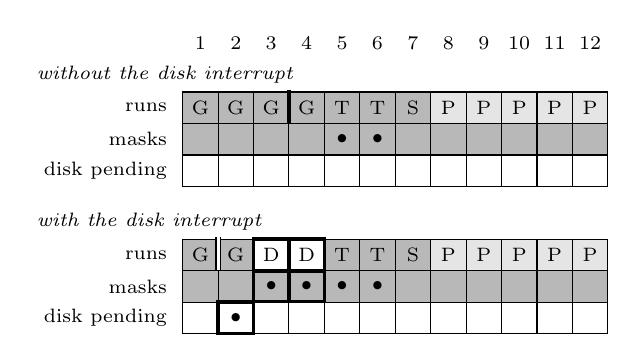
\begin{tikzpicture}[font=\scriptsize,
  cell/.style={draw, minimum width=0.45cm, minimum height=0.4cm, inner sep=0pt},
  pub/.style={cell, fill=black!28}, priv/.style={cell, fill=white},
  cG/.style={pub}, cT/.style={pub}, cS/.style={pub}, cP/.style={cell, fill=black!10},
  cD/.style={priv}, cN/.style={priv},
  head/.style={anchor=west, font=\scriptsize\itshape},
  diff/.style={draw, line width=1.3pt, minimum width=0.45cm, minimum height=0.4cm},
  irq/.style={line width=1.6pt},
  dsk/.style={double, double distance=1.1pt, line width=0.55pt}]
\foreach \i in {1,...,12} \node at (0.45*\i, 0.4) {\i};
% without the disk interrupt
\node[head] at (-1.75,0.00) {without the disk interrupt};
\node[anchor=east] at (0.15,-0.42) {runs};
\foreach \c [count=\i] in {G,G,G,G,T,T,S,P,P,P,P,P} \node[c\c] at (0.45*\i,-0.42) {\c};
\draw[irq] (1.575,-0.19) -- (1.575,-0.65);
\node[anchor=east] at (0.15,-0.82) {masks};
\foreach \c [count=\i] in {{},{},{},{},{$\bullet$},{$\bullet$},{},{},{},{},{},{}} \node[pub] at (0.45*\i,-0.82) {\c};
\node[anchor=east] at (0.15,-1.22) {disk pending};
\foreach \c [count=\i] in {{},{},{},{},{},{},{},{},{},{},{},{}} \node[priv] at (0.45*\i,-1.22) {\c};
% with the disk interrupt
\node[head] at (-1.75,-1.87) {with the disk interrupt};
\node[anchor=east] at (0.15,-2.29) {runs};
\foreach \c [count=\i] in {G,G,D,D,T,T,S,P,P,P,P,P} \node[c\c] at (0.45*\i,-2.29) {\c};
\foreach \i in {3,4} \node[diff] at (0.45*\i,-2.29) {};
\draw[irq] (1.575,-2.06) -- (1.575,-2.52);
\draw[dsk] (0.675,-2.06) -- (0.675,-2.52);
\node[anchor=east] at (0.15,-2.69) {masks};
\foreach \c [count=\i] in {{},{},{$\bullet$},{$\bullet$},{$\bullet$},{$\bullet$},{},{},{},{},{},{}} \node[pub] at (0.45*\i,-2.69) {\c};
\foreach \i in {3,4} \node[diff] at (0.45*\i,-2.69) {};
\node[anchor=east] at (0.15,-3.09) {disk pending};
\foreach \c [count=\i] in {{},{$\bullet$},{},{},{},{},{},{},{},{},{},{}} \node[priv] at (0.45*\i,-3.09) {\c};
\foreach \i in {2} \node[diff] at (0.45*\i,-3.09) {};
\end{tikzpicture}
\caption{The ordinary policy on the concrete system of \cref{sec:designs}, without and with a disk interrupt: who runs at each step (G: public user, P: private user, S: scheduler, T, D: timer and disk handler), and the state in which the step takes place ($\bullet$: set). Shading as in \cref{fig:system}: public cells shaded. A solid bar marks the timer interrupt, a hollow bar the disk interrupt; framed cells differ between the two runs. The disk handler takes steps 3 and 4 from the public user and holds the masks set meanwhile, so the runs differ in public cells. Both runs are proved traces, and the states are computed by the model's own transition (\protect\mechfile{theories/models.v}{models.v}, Section 11).}
\label{fig:run-ordinary}
\end{figure}
